The availability of tools greatly impacts the future of ideas.
Charles Babbage was the first to conceptualize the design of a computer in 1837, however, he could not implement it because the required funding and technologies needed for the production of his \emph{Analytical Engine} were not yet available.
Only in 1941, technological progress allowed for the first general-purpose computer named \emph{Z3} to be assembled.
Furthermore, it was the development of the X-ray crystallography technique that allowed Rosalind Franklin to take a picture of the crystallized fibers in 1952 that ultimately led to the discovery of DNA sequencing.
Frequently, the development of tools for a certain scientific area is an essential catalyst for progress.


In my dissertation, I implement and experiment with some of the algorithms available for the formal classes of \emph{subregular languages and mappings} that recently proved themselves to be extremely useful for modeling natural language dependencies.
Namely, I discuss the results of the automatic extraction of subregular grammars from data exhibiting various linguistic patterns, such as word-final devoicing, harmony systems of different types, and others.
The code behind the inference algorithms is available as a part of my package \emph{SigmaPie} \href{https://pypi.org/project/SigmaPie/}{\faCube} \citep{sigmapie}.
This package is open source, implemented in Python 3, and available via \texttt{pip}.
\emph{SigmaPie} allows linguists and formal language theorists to assess possible applications of subregular ideas in the areas of typology, cognitive linguistics, and natural language processing.
This package is flexible and can be used to explore a variety of research questions.
It provides researchers who are interested in subregular complexity and learning with a sandbox where they can play with new ideas in a hands-on fashion.

This thesis is meant to be a starting point for scientists who wish to incorporate \emph{SigmaPie} into their research.
It discusses the theoretical foundations of subregular linguistics and it shows how \emph{SigmaPie} can be used to experimentally test theoretical claims.
Both the discussion and the experiments consider only string representations, rather than autosegmental or tree-based ones.
That does not mean that the subregular view, or its implementation via \emph{SigmaPie}, cannot be extended to handle these richer types of structures.
Strings provide an accessible starting point for subregular work, they are not its intended endpoint.
Similarly, \emph{SigmaPie} is a sandbox rather than a finished product --- its active use in research will greatly shape \emph{SigmaPie} and push it in whatever direction turns out to be most fertile and productive.


\section{Subregular linguistics and learning}


Formal tools help to generalize natural language patterns and study them independently of linguistic theories, therefore allowing researchers to focus on one of the core questions of linguistics: \emph{what is the complexity of natural language?}
Although this question is not yet answered, we already know to some extent the complexity of the restrictions that phonotactics and morphotactics impose on the surface forms of their objects.
We have also come closer closer to understanding what types of changes are involved in phonological and morphological processes.
\textbf{Formal language theory} provides a perspective on modeling natural language dependencies.
Under this perspective, a formal language is a possibly infinite set of words satisfying some set of rules.
\emph{Subregular languages} have weak generative capacity, and therefore cannot express some types of dependencies, but their power is enough for phonology and morphology.


The subregular perspective has a goal of identifying weak subclasses of languages and mappings that are sufficiently powerful for natural language dependencies.
Subregular languages are a good git for phonotactics and morphotactics, while subregular mappings provide a convenient way to describe phonological and morphological phenomena.
These languages and mappings are subclasses of finite-state automata and transducers that are sub-divided from regular languages since the 1970s \citep{McNaughtonPapert1971}.
Although they are not novel for the field of formal language theory, they made their way to linguistics much later \citep{Heinz10ldp,Heinz11part1}.
The subregular approach is a fruitful and promising research direction, see Section 1.2 and Background for formal definitions and further information.


However, in natural language processing (NLP), little attention is paid to the vast body of linguistic research on the types of dependencies that occur in language.
Moreover, it is not even clear how to incorporate this linguistic knowledge into currently used NLP models.
Neural networks, which are widely employed nowadays in NLP, learn patterns in an uninterpretable fashion; as a result they do not furnish a way for linguists to look inside those networks and understand \emph{how} and \emph{what exactly} was learned.
On the contrary, \emph{subregular} learning algorithms (which I will call ``subregular learners'' from here on) are fully transparent and interpretable.


Subregular learning algorithms guarantee the interpretability of the way the grammar was discovered, as well as the interpretability of the grammar per se.
In other words, it is always \emph{possible to look inside the algorithm}.
Observing the behavior of the algorithm and studying its properties is necessary for understanding which configurations in the training data help to discover the pattern.
If we are dealing with natural language data, transparent learning algorithms might help to explore the way humans learn languages, to the extent that useful parallels can be drawn between the two.
Interestingly, the discussed classes of subregular languages are learnable just from positive data, without any need for negative data.


In the field of formal languages, theoretical achievements are not always followed by their practical applications.
As a result, a frequent situation arises where a learning algorithm is proposed in the literature but is not implemented.
Although it is important to prove theorems about the convergence of such algorithms, it is also important to subject them to empirical testing.
As of now, not a lot of such algorithms are implemented, and even fewer of them are employed in practice.
Sometimes, as \cite{GildeaJurafsky1996} show in their paper, the grammatical inference algorithms need to be modified and \emph{linguistically ``biased''} to work with raw language data.
The last few decades brought us a lot of new knowledge about the complexity of human language patterns, and the majority of this knowledge is still waiting to be incorporated into these algorithms.


The \emph{SigmaPie} package implements subregular learners that efficiently extract grammars after observing a finite number of well-formed strings of the target language.
This package also implements sample generators, scanners, and some other tools.
The generation of a data sample of the required complexity is needed during the design of artificial learning experiments.
Scanners and re-writers verify the well-formedness of strings regarding some grammar or modify the input according to a specified set of rules.
Additionally, the toolkit provides functions such as changing the polarity of the grammar or removing uninformative elements from the grammar.
The subregular perspective is transparent and interpretable, but so far it lacked tools that help to leverage this transparency.
Such a toolkit would be especially useful to linguists working on modeling natural language dependencies.


\section{Linguistic motivation behind the subregular approach}

What is the minimum generative capacity of the grammar that is capable of encoding human language-like patterns?
In other words, what types of dependencies must that grammar take into account?
Answering these questions might furnish powerful insights into human cognition.
The first step must be uncovering what \emph{types} of patterns do human languages exhibit.


To describe and generalize phenomena observed in natural languages, we need to build their computational or mathematical models.
Formal languages provide a way to do this.
Their object can be any structured object formed from a finite collection of discrete elements, where those objects can be strings, trees, or graphs.
In this thesis, however, I will only focus on string representations.


Subregular modeling provides two perspectives: modeling well-formedness conditions as languages, and modeling transformations as mappings.
A \textbf{well-formedness condition} can be encoded as a language, or a potentially infinite collection of strings satisfying that condition.
For example, in Russian, voiced obstruents become voiceless at the end of the word.
It results in words such as \emph{lo[b]} being excluded from the collection of well-formed Russian strings, whereas their voiceless counterparts such as \emph{lo[p]} `forehead' are grammatical.
Suppose that every word has a dedicated marker \eow~ at the end of the word.
Then the ban against voiced obstruents at the end of the word can be encoded as a grammar that rules out all cases where a voiced obstruent is followed by that marker: \emph{b\eow}, \emph{g\eow}, \emph{d\eow}, etc.


In contrast, a \textbf{transformation} can be formalized as a collection of pairs of strings, where those strings represent the states ``before'' and ``after'' the rule application.
In other words, those pairs demonstrate the underlying representations and the corresponding surface forms.
From this perspective, Russian word-final devoicing can be viewed as a collection of pairs, where the final obstruent of the first string can be either voiced or voiceless, but it is always voiceless in the second one: \emph{(lo[b], lo[p])} `forehead', \emph{(lu[g], lu[k])} `meadow', \emph{(lu[k], lu[k])} `onion', etc.
The corresponding grammar then looks at every symbol of the underlying representation and rewrites it as is, unless that symbol is the word-final voiced obstruent: then it is substituted by its voiceless counterpart.
In such a way, subregular models can capture well-formedness conditions, and encode the mapping of underlying representations to the corresponding surface forms.


In the domain of string languages, \textbf{\emph{regular languages and mappings}} provide a reasonable upper bound for phonology and morphology \citep{Johnson1972,Koskenniemi1983,KaplanKay94,BeesleyKartunnen03}.
The class of regular languages, however, can be further subdivided into a nested hierarchy of weaker \textbf{\emph{subregular}} languages.
Closer research of phonological and morphological patterns shows that in fact, these patterns do not require the whole power of regular languages.
Several subregular classes express well-formedness conditions imposed by phonotactics and morphotactics \citep{HeinzRawal11,AksenovaEtAl16,Heinz-2018-CNPG}.
Subregular --- namely, \emph{subsequential} --- mappings describe a multitude of morphological and phonological processes \citep{Chandlee2017,ChandleeHeinz2018}.
Subregular grammars found their applications even in the areas of syntax and semantics. \citep{DeSantoGrafDrury2017,GrafShafiei19SCiL,Graf19AC}.
In this thesis, I focus on modeling phonological dependencies of different kinds.


Nowadays, researchers work on many aspects of subregular languages.
There has been significant progress in the understanding of their underlying mathematical structures \citep{Fu2011,HeinzRogers2013}.
Multiple papers show how different linguistic phenomena can be accounted for in terms of subregular models \citep{HeinzRawal11,Heinz-Lai-2013-VHS,Chandlee2014,AksenovaEtAl16,DolatianHeinz2018,Graf19AC,Karakas2020}.
The approach was extended to trees and now can express such complicated dependencies as c-command or case assignment as well  \citep{GrafShafiei19SCiL,VuEtAl19SCiL}.
The works cited above are all very recent.
To help accelerate this currently growing direction of research, I implemented a package that provides the subregular functionality and explored \emph{practical} capabilities of those algorithms.


\section{Main insights and structure of the dissertation}

Different subregular learners capture different types of natural language dependencies.
While these distinct learning algorithms all rest on a sound theoretical foundation, it is unknown how well the theorems about the correctness of those learners carry over to real-world performance.
This thesis demonstrates how this open issue can be explored with the help of \emph{SigmaPie}.
I design multiple artificial learning experiments and score the subregular learners on datasets exhibiting patterns such as local assimilations, multiple long-distant harmonies of different types, some typologically unattested patterns, and others.
The datasets range from artificial automatically generated samples to real-language datasets such as German, Finnish, and Turkish wordlists.
While the artificially generated datasets explore if a pattern is learnable in general, the raw data shows what issues the learners have when faced with the raw natural language data.
Every target pattern is approached from two perspectives: as a well-formedness condition on the surface forms, and as a transformational rule changing values of some elements.


\paragraph{Specific findings}
I show that indeed, subregular learners perform as theoretically expected, and extract grammars of the corresponding complexity from generated datasets.
It confirms that they can model different natural language dependencies, including but not limited to local dependencies, different long-distance harmonies, and even segmental patterns.
Importantly, some of these learners were able to perform well on such complex tasks as learning of a long-distance dependency from raw data.

\paragraph{Relevance for linguistics}
Subregular languages and mappings indeed model a wide variety of natural language patterns.
Subregular learning algorithms efficiently learn languages and mappings from positive data.
Setting up the learning pipeline itself is not complicated, and I thoroughly discuss the way I did it in my thesis.
Such \emph{SigmaPie}-based learning experiments provide a way to test ideas on artificial and natural language datasets.
\medskip


While chapters 3 and 4 explore subregular modeling from a practical point of view, \textbf{Chapter 2.\ Background} gives a theoretical perspective on subregular languages and mappings.
I discuss the modeling capacities of subregular grammars and transformations by capturing attested natural language patterns such as word-final devoicing, unbounded tone plateauing, and several different types of harmonies.
Namely, the reviewed formal classes are strictly local, strictly piecewise, tier-based strictly local, and multi-tier strictly local languages; and subsequential transformations.
Additionally, in that chapter, I also discuss the problem of inferring grammars from data, and list the useful properties shared by the subregular learners.



In \textbf{Chapter 3.\ Learning languages}, I target modeling well-formedness conditions.
Namely, I employ four subregular language classes that express generalizations, including local and long-distance processes such as attested and unattested harmony systems with and without blockers, word-final devoicing, and even suprasegmental patterns.
A training sample is a list of well-formed strings that does not include words that violate the target generalization.
So, for example, for a target pattern of vowel harmony, the training dataset is a sample of harmonic words.
The conducted experiments confirmed the learning expectations for the artificial datasets, showing how different linguistic patterns are captured by subregular models.
However, the performance of the learners on raw natural language data was worse, and in some cases, a more powerful model was required to capture a pattern of lower complexity.
In that chapter, I also outline the architectures of the learners originally introduced in \citep{Heinz-2010-SEL,JardineMcMullin2017,McMullinAksenovaDeSanto2019}.


\textbf{Chapter 4.\ Learning mappings} is concerned with modeling transformations changing the underlying representations into the corresponding surface forms.
According to \cite{Chandlee2014}, many of phonological and morphological dependencies belong to the class of subsequential mapping.
Thus, I give an overview of a subsequential learner OSTIA \citep{OncinaEtAl1993,DeLaHiguera2010}, and use it to extract generalizations from datasets exhibiting different linguistic dependencies.
In this case, patterns are represented as pairs of strings.
So, for example, if a pair demonstrates a vowel harmony, then the first string shows the underlying, or underspecified, representation, while the vowels in the second word are fully specified and harmonic.
The learner was able to model a variety of local and long-distance dependencies but struggled to capture a blocking effect.
Additionally, that chapter discusses other algorithms that learn mappings and can be employed for similar tasks in the future.


Finally, \textbf{Chapter 5.\ Conclusion} summarizes the obtained results and proposes directions for future research.
Figure \ref{chaptersstructure} gives an overview of the flow of this thesis, starting from the theory of modeling well-formedness conditions and transformations, and then followed by a part discussing the applications and the accomplished learning experiments.
The \emph{SigmaPie} package was used in the experiments reported in Chapters 3 and 4.
Its code is available via Python package manager \texttt{pip} and is listed in Appendix A.
The correctness of the code was assessed via a series of unit tests, provided in Appendix B.

This dissertation shows how learning experiments can be conducted using subregular learners from \emph{SigmaPie} package and discusses the results of those experiments.
This package contains functionality that allows linguists to model linguistic phenomena and test those models, manually and automatically.
	

\begin{figure}[h!]
\centering
\tikzset{every picture/.style={line width=0.75pt}} %set default line width to 0.75pt        
\resizebox{\linewidth}{!}{%
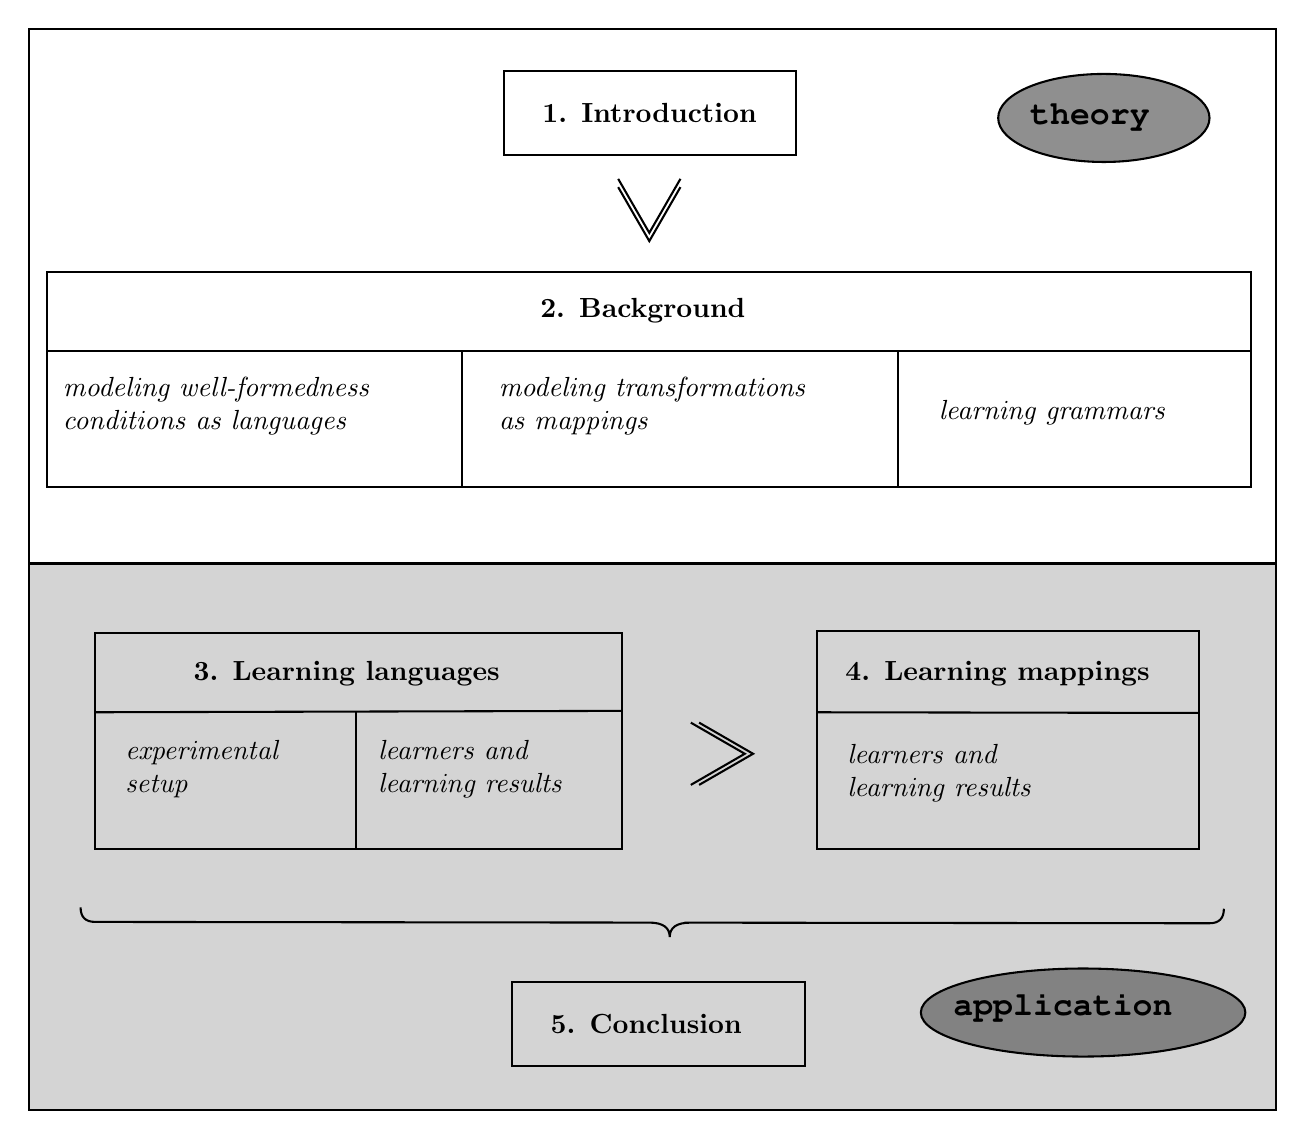
\begin{tikzpicture}[x=0.75pt,y=0.75pt,yscale=-1,xscale=1]
%uncomment if require: \path (0,538); %set diagram left start at 0, and has height of 538

%Shape: Rectangle [id:dp8221412876102787] 
\draw   (250,31) -- (390.83,31) -- (390.83,71.33) -- (250,71.33) -- cycle ;
%Shape: Rectangle [id:dp5026563864255413] 
\draw   (29.83,128) -- (609.83,128) -- (609.83,231.33) -- (29.83,231.33) -- cycle ;
%Straight Lines [id:da7513846337736221] 
\draw    (29.83,166) -- (609.83,166) ;
%Shape: Rectangle [id:dp8727441659717616] 
\draw   (52.83,302) -- (306.83,302) -- (306.83,406) -- (52.83,406) -- cycle ;
%Straight Lines [id:da08433324969296474] 
\draw    (52.83,340) -- (306.83,339.33) ;
%Shape: Rectangle [id:dp7150794601993389] 
\draw   (400.83,301) -- (584.83,301) -- (584.83,405.67) -- (400.83,405.67) -- cycle ;
%Straight Lines [id:da1691060851390651] 
\draw    (400.83,340) -- (584.83,340.33) ;
%Straight Lines [id:da8740251300311048] 
\draw    (229.83,166) -- (229.83,232) ;
%Straight Lines [id:da7832612810103501] 
\draw    (439.83,166) -- (439.83,232) ;
%Straight Lines [id:da3202514288331062] 
\draw    (178.83,340) -- (178.83,406) ;
%Shape: Rectangle [id:dp5815929836430904] 
\draw   (254,470) -- (394.83,470) -- (394.83,510.33) -- (254,510.33) -- cycle ;
%Shape: Rectangle [id:dp21095701304766612] 
\draw   (21,10.67) -- (621.83,10.67) -- (621.83,531.67) -- (21,531.67) -- cycle ;
\draw   (335,83) -- (320,109) -- (305,83)(335,87) -- (320,113) -- (305,87) ;
\draw   (340,345) -- (366,360) -- (340,375)(344,345) -- (370,360) -- (344,375) ;
%Shape: Brace [id:dp7711459734646808] 
\draw   (46,434) .. controls (45.99,438.67) and (48.32,441) .. (52.99,441.01) -- (319.84,441.33) .. controls (326.51,441.34) and (329.84,443.68) .. (329.84,448.35) .. controls (329.84,443.68) and (333.17,441.35) .. (339.84,441.36)(336.84,441.36) -- (589.82,441.66) .. controls (594.49,441.67) and (596.82,439.34) .. (596.83,434.67) ;
%Shape: Rectangle [id:dp23976569225238542] 
\draw  [fill={rgb, 255:red, 0; green, 0; blue, 0 }  ,fill opacity=0.17 ] (21,268.33) -- (621.83,268.33) -- (621.83,531.67) -- (21,531.67) -- cycle ;

% Text Node
\draw (267,45) node [anchor=north west][inner sep=0.75pt]   [align=left] {\textbf{1. Introduction}};
% Text Node
\draw (266,139) node [anchor=north west][inner sep=0.75pt]   [align=left] {\textbf{2. Background}};
% Text Node
\draw (36,177) node [anchor=north west][inner sep=0.75pt]   [align=left] {\textit{modeling well-formedness}\\\textit{conditions as languages}};
% Text Node
\draw (246,177) node [anchor=north west][inner sep=0.75pt]   [align=left] {\textit{modeling transformations}\\\textit{as mappings}};
% Text Node
\draw (458,188) node [anchor=north west][inner sep=0.75pt]   [align=left] {\textit{learning grammars}};
% Text Node
\draw (98.98,314) node [anchor=north west][inner sep=0.75pt]   [align=left] {\textbf{3. Learning languages}};
% Text Node
\draw (66.07,352) node [anchor=north west][inner sep=0.75pt]   [align=left] {\textit{experimental}\\\textit{setup}};
% Text Node
\draw (187.9,352) node [anchor=north west][inner sep=0.75pt]   [align=left] {\textit{learners and}\\\textit{learning results}};
% Text Node
\draw (412.98,314) node [anchor=north west][inner sep=0.75pt]   [align=left] {\textbf{4. Learning mappings}};
% Text Node
\draw (413.9,354) node [anchor=north west][inner sep=0.75pt]   [align=left] {\textit{learners and}\\\textit{learning results}};
% Text Node
\draw (271,484) node [anchor=north west][inner sep=0.75pt]   [align=left] {\textbf{5. Conclusion}};
% Text Node
\draw  [fill={rgb, 255:red, 0; green, 0; blue, 0 }  ,fill opacity=0.44 ]  (539, 53.67) circle [x radius= 50.91, y radius= 21.21]   ;
\draw (502,45) node [anchor=north west][inner sep=0.75pt]  [font=\large,color={rgb, 255:red, 0; green, 0; blue, 0 }  ,opacity=1 ] [align=left] {{\large {\fontfamily{pcr}\selectfont \textbf{theory}}}};
% Text Node
\draw  [fill={rgb, 255:red, 0; green, 0; blue, 0 }  ,fill opacity=0.39 ]  (529, 484.67) circle [x radius= 78.18, y radius= 21.21]   ;
\draw (465,474) node [anchor=north west][inner sep=0.75pt]  [font=\large,color={rgb, 255:red, 0; green, 0; blue, 0 }  ,opacity=1 ] [align=left] {\textbf{{\large {\fontfamily{pcr}\selectfont application}}}};

\end{tikzpicture}
}
\caption{Flow of chapters of this dissertation: Introduction, Background, Learning languages, Learning mappings, and Conclusion.}
\label{chaptersstructure}
\end{figure}


